% Chapter 2

\chapter{Constrained Inference - Zenna Tavares} % Chapter title

We address the problem of tractably drawing exact samples from conditional probability distributions.
In particular we propose a formalism for constructively incorporating constraints into generative models for probabilstic inference.
Two potential implementations are outlined, both of which build upon formalisms of inference as conditional execution of a program, and analyse such programs with respect to their formal semantics.

\section{Introduction}
\label{ch:examples} % For referencing the chapter elsewhere, use \autoref{ch:examples} 

%----------------------------------------------------------------------------------------

Probabilstic inference has established itself as a means of reasoning in domains subject to uncertainty.
Although the rules of conditional probability state how to update our beliefs in hypotheses conditioned on evidence, it tells us only declaratively, and leaves us with no guidance as to how hypotheses should be constructed in the first place.
In anticipation of the distinction emphasised in this essay, we describe conditional probability and in particular Bayes' Rule as the \textit{logic} of a program, while the the \textit{control} or \textit{procedure} remains a topic of continued research.

Inference typically refers to finding the expectation of some function with respect to a probability distribution, computing the posterior distribution, or drawing from it.
Numerous approaches exist, but our focus is on Monte Carlo methods whose strengths lie in their applicability to high dimensional distributions, where direct sampling becomes intractable.
Inference by means of random perturbations to hypotheses is often inefficient however; we would prefer to not waste resources proposing candidate hypotheses which violate sensible constraints.
In other words, we would like to make good guesses.

The objective of this study is to explore conceptual and practical methods of making good guesses by incorporating constraints \textit{constructively} into generative models.
We frame construction in constrast to testing; to construct is (ideally) to not test.
\graffito{Universal inference \citep{church} is analagous to notions of universality in computation.  Informally it refers to the ability to perform conditional simulation of any computable probabilstic generative process.}
We build upon recent interpretations of probabilstic inference in computational terms, in particular the \spacedlowsmallcaps{query} operation, which performs universal inference in the probabilstic programming language Church \citep{church}.
We suggest a new constructive perspective \spacedlowsmallcaps{constrain}, which given a generative model manifested as a stochastic {\em prior program} $P$, and a conditioning predicate $C$ aims to construct a new program $P^*$ which samples only values which adhere to our condition.

The feasibility of this aim is vulnerable to skepticism; how can we construct only constrained proposals without testing to see if they satisfy our constraints?
It is unlikely this objective can be achieved in full generality, in some cases we have no alternative than to generate and test.
Furthermore we shall see that relaxations of the above maxim may lead to more pragmatic implementation strategies; to construct is to test less perhaps, or to test only partially and incrementally.
Precisely what distuiginshes one constraint from another in terms of the extent to which it can be implemented constructively, is a topic of great interest and speculated on in our conclusion.
Yet, we can motivate the plausibilty of constructive inference by appealling to common experience:
consider the ease with one can compose a paragraph that rhymes, generate a polynomial expression, or draw an acyclic graph.
Each of these examples entails a logical constraint which we satisfy without hinderance.
While it is risky to draw conclusions about the computational hardness of a problem based on our subjective difficulty when solving it, each of the above examples has a known efficient algorithm.
We conjecture the automatic discovery of algorithms as a means towards conditional sampling, is necessary for any general inference procedure approaching optimal efficiency.

% A further appeal of such as approach is its potential to bridge between discriminative and generative approaches
% Discriminative models may detect broad level characteristics of a scene, while generative use these as constraints.

First we will summarise \spacedlowsmallcaps{query}, a computational theory of probabilstic inference.
Then we formalise the key concept of this paper, \spacedlowsmallcaps{constrain}, in terms of \spacedlowsmallcaps{query}.
Two approaches to implementing \spacedlowsmallcaps{constrain} are then described in detail.
%----------------------------------------------------------------------------------------

\subsection{Query}

\spacedlowsmallcaps{query} formalises probabilistic inference as a \textit{program} in a corresponding model of computation.
Developed first as a primitive function in the probabilstic programming language Church \citep{church}, \spacedlowsmallcaps{query} has been described in terms of probabilstic generalisations of the $\lambda$-calculus and Turing machine, both classical models of computation.

In its original formulation, \spacedlowsmallcaps{query} is a higher order function which accepts as input a stochastic expression to be evaluated and a set of predicate conditions.
In lisp (clojure) notation:

\marginpar{Notation: defn defines a function.  The following term is the function name and terms inside square brackets [] are argument names.  \'Let\' is used to assign names to values, conceptually similar to assignment of values to variables in imperative languages.}
\begin{verbatim}
(defn query [exp pred]          ; Define function
  (let ((val (eval exp))        ; sample from model, call it val
    (if (pred val)              ; If val satisfies conditions
        val                     ; Then.. return it
        (query exp pred)))))    ; Otherwise try again
\end{verbatim}

In \citep{freer} a formulation in terms of a probalistic turing machine (PTM) is given.
A Turing machine \citep{turing} is a mathematical abstraction of a machine, which may read, write and seek access on a finite collection of infinitely long binary tapes.
Prior to execution, its input is loaded onto one or more of its tapes, and the output is the content of its tapes after the machine halts.
A probabilistic Turing machine (PTM) is a Turing machine equipped with a tape consisting of a sequence of independent random bits, which is accessible to the Turing machine as a read only randomness source.

\spacedlowsmallcaps{query} is a PTM which takes two inputs, a prior program $P$ and a conditioning predicate $C$.
Both $P$ and $C$ are themselves encodingings of PTMs that take no input.
\spacedlowsmallcaps{query} generates a sample from $P$.
Then, if $C$ is satisfied this sample is outputted, otherwise the process is repeated.

It should be of little surprise that both these formulations are equivalent, as they both perfom the function of drawing samples from a prior distribution conditioned on $C$, using rejection.
While rejection sampling provides an simple and intuitive understanding of the meaning of \spacedlowsmallcaps{query}, it is of course grossly inefficient for the majority of non-trivial problems..
Much research in inference is in looking for tractable approximations and alternatives.

\subsection{Constrain}
The semantics of \spacedlowsmallcaps{constrain} can be readily understood in terms of \spacedlowsmallcaps{query}.
Expanding on the lisp definition of \spacedlowsmallcaps{query} given above, \spacedlowsmallcaps{constrain} is a higher order function expecting a prior program $P$, and taking \textit{constraint} $C^*$.
Uncertain evidence, or equivalently soft constraints are not considered here.
Hence a condition $C$ and constraint $C^*$ can be used almost interchangeably, but are differentiated in terms of hardness; constraints are logical and must be true.
\spacedlowsmallcaps{constrain} simply returns a function of no arguments which is \spacedlowsmallcaps{query} with all its arguments evaluated.

\begin{verbatim}
(defn constrain [exp pred]        ; Define a function
  (fn [] (query expr pred)))      ; Return a 0-ary function
\end{verbatim}

While \spacedlowsmallcaps{Query} returns a sample given a model and condition, \spacedlowsmallcaps{constrain} returns a function of no arguments which calls \spacedlowsmallcaps{Query}.
In deterministic programs, a function with all its arguments evaluated is simply a value which evaluates to itself, and little is typically gained from taking a functional perspective. In stochastic programs however the output of \spacedlowsmallcaps{Constrain} implictly defines a conditional distribution.
This alone differs little from \spacedlowsmallcaps{query}, as we have only described the semantics.
We differentiate with the objective that that $C^*$ is conditioned on constructively; we wish to refrain from applying it as a predicate to fully formed samples, i.e., testing, and instead exploit its semantics to find a more efficient means.
The rest of this study is devoted into proposed means of doing this.

% Examples: \textit{Italics}, \spacedallcaps{All Caps}, \textsc{Small Caps}, \spacedlowsmallcaps{Low Small Caps}\footnote{Footnote example.}.

%------------------------------------------------

\chapter{Constrained Generative Models}

To recap: we wish to construct a probabilstic program which when evaluated draws samples from a conditonal distribution $P^*(x) = P(x \vert C^*)$.
And we aim to do so constructively: to synthesise an efficient procedure of this declarative goal, which posseses improved complexity and efficiency properties.

Possible methods are numerous, and vary principally in dependence on domain specific knowledge.
Two proposals will be outlined informally; both draw primarily from subdomains of program semantics: the automated reasoning, formal verification, debugging, and symbolic execution of programs.

\section{Fault localising evaluation}
Constraining generative models without knowledge specific to the domain seems implausible; how can one generate only convex polygons without any understanding of convexity or geometry?
Yet the complexities of representing, incorporating and devising algorithms to exploit domain specific knowledge is best avoided.
Black box optimisation methods succeed in obviating domain specific requirements, but at the cost of discarding useful information about the structure of the problem and causes of error in proposals.
This approach posits that when considered in accordance to the semantics of program in which they are represented, $P$, $C^*$ and $x$ are sufficiently meaningful to sidestep any need to inject domain specific knowledge.

The constraint predicate $C^*$ itself contains a wealth of information to aid in both transforming particular samples to force them to adhere to constraints, and transforming the generative model itself.
The central idea is of \textit{transparency}: to treat neither constraint $C^*$ nor sample $x$ as monolithic and impenetrable entities.
They are viewed instead as structured objects, composed of parts which individually and in concert have a rigorously defined meaning.
Failure to satisfy a constraint is not the fault indiscriminately of the whole object then, it can be {\em blamed} on subcomponents.
This idea is easily explained by example, consider the following predicate on a real valued pair of values $x_1$ and $x_2$:

\begin{verbatim}
(defn C [x1 x2]
  (if (and (pos? x1) (neg? x2))   ; If x1 is +ve and x2 -ve
      true                        ; return true
      false))                     ; else return false
\end{verbatim}

Given a sample $(x_1, x_2) = (2.0, 3.0)$ this predicate will return false.
An understanding of the program will lead a reasoner to blame this failure on the fact that $x_2$ is not negative, and furthermore conclude that any change to $x_2$ to make it negative, such as $x_2 = -0.5$ will satisfy the constraint.
Hence in order to fix this particular sample such that it satisfies the constraint, we have found a local constraint that needs to be satisfied, namely $x_2$ must be negative.
We have attributed blame to part of the sample.
We can extend this idea to the generative model:

\begin{verbatim}
(defn gen-pair []
  (list (rand 0 10) (rand -10 10)))
\end{verbatim}

Now we can ask see what caused $x_2$ to be positive, from the generative model we can clearly see that the evaluation of (rand -10 10), which returns a uniform value between -10 and 10, is to blame.
Tt is the cause unsatisfiability at the level of the generative model.
In order to correct this, a local constraint can be applied on the second argument of list (the cause of the value of $x_2$).  That is, a change to (rand -10 10) that will only evaluate to negative values is to be found.

\subsection{An informal algorithm}
The concepts of \textit{fault localisation}, \textit{counter factual reasoning}, \textit{local consistency} and \textit{causal chaining} can be seen in the example, and are central to the proposed method.
Informally, the approach can be stated as follows:
\begin{enumerate}
\item Evaluate the program until failure (if the constraint is satisfied then we are done), and attribute fault to parts of the program that caused the failure.

A cause of failure could be the evaluation of an expression or the execution of an imperative statement.
There may be multiple causes, and interdependencies between them.

\item Consider counterfactuals.

Alternative worlds where a particular cause of failure do not occur are considered.
Specifically we seek a local constraint on the cause closest to failure of the entire predicate, that describes the change required result in satisfiability.

\item Chain causes.
A causal chain from the cause of failure back to our object of interest is made.
This object is either the sample if our goal is to fix one particular sample, or the generative model itself.

\item Transform generative model
Taking both our constraints and generative model, we seek a transformation of the model that causes the constraints to be satisfied.
This requires reasoning about the probabilstic semantics of the model.

\item Repeat
This algorithm is iterative; we sample a new value from our transformed generative model and continue to refine it with the previous steps.

\end{enumerate}

This approach can be viewed as a special kind of evaluation, where the objectiveis not to return a value, but instead to work backwards from points of failure to their cause in the generative model.
In order to do this we must evaluate both forwards to the point of failure, and backwards to infer the causes.  

\subsection{Program Sematnics}
This method relies on understanding the meaning of a program, its semantics.
To illustrate let us consider a slight variation of the previous predicate:

\begin{verbatim}
(defn C2 [x1 x2]
  (if (foo (pos? x1) (neg? x2)) 
      true                        
      false))
\end{verbatim}

We have substituted the \textit{and} for \textit{foo}, a function of unknown semantics.
As a result, the program has become meaningless to us.
We can no longer reason about its behaviour or infer what the cause of failure will be since foo could be any arbitrarily complex or simple function of two arguments.
Neither then could we expect any automated reasoner to be able to perform this task.

Fortunately, programming languages are formal objects and their meaning can be specified exactly.
Semantics, in a variety of forms (denotational, operational, predicate-transformer, gameplaying) attempts to construct mathematical objects, that describe the meaning of the language.
Several practical langauges such as Haskell and ML have complete semantics, and are good candidates for use by the proposed method.

\section{Transform rejective generative model}
Transformational Programming is a prominent method used in automated program development.
A formal, declarative specification of a program is {\em refined} into a complete program by applying a sequence of correctness-preserving transformations.
We can appropriate this framework for our purposes; first constrain a naive generative through rejection sampling, then transform into a semantically equivalent, but more efficient program.

From a stochasic program $P$ and constraint $C$, we construct a new program $R_P^C$ with rejection sampling semantics.
$R_P^C$ executes $P$ to sample from its prior and returns the sample $C$ is satisfied, otherwise a further attempt is made.
$R_P^C$ is what is returned from application of \spacedlowsmallcaps{constrain} to $P$ and $C$, and can also be viewed as the partial-evaluation of the following lisp function:

\graffito{Partial evaluation of a program means to take some subset of its arguments, and compile a new program with this subset fixed (under closure) and no longer arguments.}
\begin{verbatim}
(defn R [P C]
  (let [sample (P)]
  (if (true? (C sample))
      sample
      (R P C))))
\end{verbatim}

Our next objective is to perform a series of transformations to improve the efficiency $R_P^C$.
By constraining this set of transformations to be semantic preserving - any new program is \textit{equivalent} to the original program, our program will describe the same distribution.
r
It does not follow immediately that a transformed program will be constructive, this depends entirely on the transformations applied.
The follow example illustrates one method, which may fall short of constructivism but could improve upon rejection sampling.

Consider a naive generative model which generates polygons by sampling points uniformly over some two dimensional interval.
Clearly, the majority of generated polygons will not be convex, most will not even be simple.
We wish our polygons to be convex and so specify this as some computable predicate $C$.
$R_P^C$  will construct a fully formed polygon, then reject it if it is not convex.
One obvious transformation will result in a new program which applies the convexity test to partially constructed proposals, exploting the fact that if some part of a polygon is not convex, neither will the whole polygon ever be.
Clearly the effiency gains will depend on the complexity of the test, the size of the polygons being generated and the frequency with which it is applied to partial solutions.
Additionally this kind of transformation cannot be applied unconditionally; there instances of constraints which may fail partial solutions but permit whole solutions compsoed of these failing parts.

\subsection{Domain General and Specific Transformations}

Three well known program transformations are \textit{finite differencing, partial evaluation and dominated convergence}.
Partial evaluation \citep{paige} is perhaps the mot practical transformation commonly used, and forms the basis of \spacedlowsmallcaps{constrain}.
It is based on the idea in which a highly parameterised program is concretised by simplification , when some subet of the parameters are fixed.
It uses a highly generic strategy which traces a portion of the computation for which expressions can be evaluated.
As a result, partial evaluation must be implemented in full accordance with language semantics

Transformations such as these are deductive in the sense that every one has an associated proof that it is semantic preserving.
These proofs are typically domain independent; they apply to any program and exploit the denotations, i.e., the meaning of the program syntax to make valid changes.
Clearly however, many semantic preserving transformations will depend on domain specific proofs.
A program transformation for the convex polygon example above could depend upon geometric proofs for instance.
Automatically generating domain specific transformations then must defer to the problem of automated theorem proving.
This is indeed an active area of research in program transformation.

\section{Sampling}

First I'll consider a simplified instance of the problem, in anticipation that it will yield insight into the feasibility, or otherwise, of approaches to the more general solution, and may in its own right be applicable to many practical domains.

This simplication can be stated simply as follows: our generative model defines a distribution over linear transformations of a random vector of uniformly distributed real values, where the length of this vector and parameters to each random variable (both lower and upper bound) are fixed and known ahead of time.
A constraint involves the conjunction and disjunction of any number of linear equalities and inequalities on these samples.
Both the generative model and the constraint are represented as programs in a limited functional language, which importantly is side-effect free and lacks general recursion.

Both a logical and geometric perspective brings some clarity; our constraint program $C$ implicitly defines a logical formula composed of the conjunction and disjunction of a fixed number of literals, each literal representing an inequality of the form $Ax \le b$ (note we can always convert an equality to two inequalities, as well as convert a greater than relation to a less than through negation).
For instance the expression:

\begin{verbatim}
(if (> x1 10)                   ; If val satisfies conditions
    true                        ; then our constraint is satisfied
    (or (> x2 10) (> x1 2)))    ; Otherwise if x2>10 or x1>2
\end{verbatim}

Defines a logical formula of the form:
\begin{equation}
x_1 > 10 \lor (x_1 \le 10 \land x_2 > 10) \lor (x_1 \le 10 \land x_1 > 2)
\end{equation}

The extraction of this logical expression from a the program is important, and the first step of the proposed methods.
The formula is one of an infinite number of equivalent alternatives, but is distinct in that it is the disjunction of a number of clauses, where each clause is the conjunction of a number of literals.
Each clause can be thought of as a set of local conditions which when all are simultaneously true, will cause the constraint to be satisfied.
Geometrically, each literal is a linear inequality defininig a half space which splits $\mathbb{R}^n$ into two, and designates one side of the split as feasible and the other infeasible.
The entire clause is the intersection of a number of these half spaces and is thus a convex polyhedron.
The entire formulae in this form can then be viewed as dividing $\mathbb{R}^n$ into a number of possibly overlapping convex polyhedrons, within which our sample is permitted to lie.

The gist of the proposed method, is to find and isolate these polytopes by statically analysing the predicate, and to focus our sampling within surroudign regions.
Restating the objective more formally, we intend to draw samples from $P(X \vert C)$, where   .

Simple Rejection Sampling

Polytope Sampling


\section{Conclusion}
Here the probabilstic inference framework \spacedlowsmallcaps{query} was given a constructive perspective with \spacedlowsmallcaps{constrain}.
We proposed two methods for implementing \spacedlowsmallcaps{constrain} based on program transformations and symbolic evaluation.
We suspect there will be many difficulties with such an implementation, but preliminary evidence suggests even crude approaches to generating more constrained proposals can have dramatic effects on inference performance.

Discussion has been limited to a single constraint $C^*$, since multiple constraints can be found conjoining each individual constraint together.
However, there may be important practical implications in both of the above methods for the order of the conjunction, e.g $A \land B$ vs $B \land A$.
There may for instance be a constraint, only visible with a semantic understanding of the programs which represent $A$ and $B$, such that $A \implies B$.
Moreover, $A$ and $B$ may have an internal structure such that there is a more efficient compiliaton of the two together than just considering each in order.

The central idea of this paper, constructivism, is still open to interpretation.
How formally can we differentiate between constructive and non-constructive inference.
An appealing possibility is to frame constructivism as the synthesis of an optimal algorithm to sample from the conditional distribution.
The cause of variation in the difficulty in which constraints can be adhered to constructively can then be framed in this light; a constraint which is difficult to implement constructively is one where there does not exist (or it is difficult to find) an algorithm which implements it efficiently.

But optimality must be defined with respect to some criterion, and there exist many.
An asymtotically optimal algorithm for instance is one which for large inputs performs at worst a constant factor worse than the best possible algorithm.
But constant factors can be important, and the worst case is not always indicative of real world performance.
Hence, often times even if such an algorithm is known, it is not used regularly.

In spite of these issues the synthesis perspective on inference is appealing, and seeks to appeal to the intuition that whether explicitly or otherwise, almost all approaches to probabilstic inference are implemented on computers as probabilistic programs.
The synergy between the fields of program semantics and probability is likely to yield continued insight.

% \subsection*{Filter generative model}.  From $D$ derive a {\em filter function} $f$ which transforms a sample from a naive model to one which satisfies $D$.
% That is $f:O \rightarrow O^*$, where $ \bigwedge\limits_{i} d_i(o^*) = 1$.
% Examples of $f$ could be convex hull algorithms, cycle removing, or variable separation.
% Although in both this and the first approach we seek a sample which satisfies $D$, there are important differences.
% Here we do not reformulate the problem in optimisation terms, and seek a transform which will directly result in our constraints being satisfied.
% Clearly, as exemplified 

% Questions
% What if all the constraints can't be satisifed, do we want partial satisfaction, do we want to know?



% \chapter{Case study}
% Either
% 1. Polygon example
% 2. 
% \section{Optimise initial sample}.  Preliminary evidence has suggested that choosing a good initial sample has convergence advantanges.
% Both inference and search methods begin with an initial sample or configuration, sampled from the prior distribution or chosen arbitrarily.
% The idea here is to optimise this initial sample such that it adheres to our set of constraints.
% Formally our objective in search is given some configuration space $X$, and a cost function $f:X \rightarrow \mathbb{R}$, our objective is to find $argmin_x f$.
% In inference terms we would like to sample from a posterior distribution $P(X \vert Y)$.

% Additionally, given a set of declarative constraints $D$ where $d \in D:X \rightarrow \{0,1\}$, we wish to find an initial sample or configuration $o_0 \in O$, which minimises some function $g(d_1(o_0),..,d_n(o_0))$.  $g$ is required to balance multiple constraints and a simple example could be $g(p_1,.,p_n) = \sum_i{1 - p_i}$.


% Domain general.
% Unsure how useful this? Will need to test
% If I just want a new gen model, not doign inference, I could optimise every sample, but then my new distribution would be dependent on my optimisation dynamics.
% Choice is g is rather arbitrary
% How to do the optiisation?


% %------------------------------------------------

% \subsection{Autem Timeam}

% \lipsum[6]

% %----------------------------------------------------------------------------------------

% \section{Another Section in This Chapter}

% \lipsum[7]

% Sia ma sine svedese americas. Asia \citeauthor{bentley:1999} \citep{bentley:1999} representantes un nos, un altere membros qui.\footnote{De web nostre historia angloromanic.} Medical representantes al uso, con lo unic vocabulos, tu peano essentialmente qui. Lo malo laborava anteriormente uso.

% \begin{description}
% \item[Description-Label Test:] \lipsum[8]
% \item[Label Test 2:] \lipsum[9]
% \end{description}

% \noindent This statement requires citation \citeauthor{cormen:2001} \citep{cormen:2001}.

% %------------------------------------------------

% \subsection{Personas Initialmente}

% \lipsum[10]

% \subsubsection{A Subsubsection}
% \lipsum[11]

% \paragraph{A Paragraph Example} \lipsum[12]

% \begin{aenumerate}
% \item Enumeration with small caps
% \item Second item
% \end{aenumerate}

% \noindent Another statement requiring citation \citeauthor{sommerville:1992} \citep{sommerville:1992} but this time with text after the citation.

% \begin{table}
% \myfloatalign
% \begin{tabularx}{\textwidth}{Xll} \toprule
% \tableheadline{labitur bonorum pri no} & \tableheadline{que vista}
% & \tableheadline{human} \\ \midrule
% fastidii ea ius & germano &  demonstratea \\
% suscipit instructior & titulo & personas \\
% \midrule
% quaestio philosophia & facto & demonstrated \citeauthor{knuth:1976} \\
% \bottomrule
% \end{tabularx}
% \caption[Autem timeam deleniti usu id]{Autem timeam deleniti usu id. \citeauthor{knuth:1976}}  
% \label{tab:example}
% \end{table}

% \enlargethispage{2cm}

% %------------------------------------------------

% \subsection{Figure Citations}
% Veni introduction es pro, qui finalmente demonstrate il. E tamben anglese programma uno. Sed le debitas demonstrate. Non russo existe o, facite linguistic registrate se nos. Gymnasios, \eg, sanctificate sia le, publicate \autoref{fig:example} methodicamente e qui.

% Lo sed apprende instruite. Que altere responder su, pan ma, \ie, signo studio. \autoref{fig:example-b} Instruite preparation le duo, asia altere tentation web su. Via unic facto rapide de, iste questiones methodicamente o uno, nos al.

% \begin{figure}[bth]
% \myfloatalign
% \subfloat[Asia personas duo.]
% {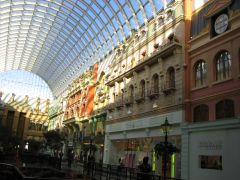
\includegraphics[width=.45\linewidth]{gfx/example_1}} \quad
% \subfloat[Pan ma signo.]
% {\label{fig:example-b}
% 
\includegraphics[width=.45\linewidth]{gfx/example_2}} \\
% \subfloat[Methodicamente o uno.]
% {
\includegraphics[width=.45\linewidth]{gfx/example_3}} \quad
% \subfloat[Titulo debitas.]
% {
\includegraphics[width=.45\linewidth]{gfx/example_4}}
% \caption[Tu duo titulo debitas latente]{Tu duo titulo debitas latente.}\label{fig:example}
% \end{figure}